%%%%%%%%%%%%%%%%%%%%%%%%%%%%%%%%%%%%%%%%%%%%%%%%%%%
%% P3: Phenomenology of Particle Physics                         
%%
%% Author:  André Rubbia                   		 
%%
%% Figure 3.7 The layout of the LEP collider and the current CERN accelerators complex to operate the LHC (PS, SPS, and LHC drawn).
%%
%% This work is licensed under the Creative Commons Attribution 4.0 International License. 
%% To view a copy of this license, visit http://creativecommons.org/licenses/by/4.0/ or 
%% send a letter to Creative Commons, PO Box 1866, Mountain View, CA 94042, USA.
%%
%%%%%%%%%%%%%%%%%%%%%%%%%%%%%%%%%%%%%%%%%%%%%%%%%%%

\documentclass[a4paper,10pt]{article}

\usepackage[T1]{fontenc}
\usepackage[utf8]{inputenc}
\usepackage{lmodern}
\usepackage[labelfont=bf]{caption}
\usepackage{upgreek}

\usepackage{tikz}
\usetikzlibrary{patterns}
\usetikzlibrary{decorations.pathmorphing}
\usetikzlibrary{decorations.markings}
\usetikzlibrary{arrows}
\usetikzlibrary{svg.path}
\usetikzlibrary{shapes}
\usetikzlibrary{arrows.meta}
% define the arrow style
\tikzset{
    arrow/.style={
        decoration={
            markings,
            mark=at position .5 with {
                \arrow[#1, scale=1.5]{latex}
            }
        },
        postaction={decorate},
    }
}
\tikzset{
    arrow flipped/.style={
        decoration={
            markings,
            mark=at position .5 with {
                \arrow[#1, scale=1.5]{latex reversed}
            }
        },
        postaction={decorate},
    }
}
\pgfkeys{/pgf/number format/.cd,1000 sep={}}\usepackage{pgfplots}
\pgfplotsset{compat=1.17}
\usepgfplotslibrary{ternary}
\usepgfplotslibrary{fillbetween}
\usepgfplotslibrary{external}

\def\d{\mathrm{d}}

\begin{document}

%%%%%%%%%%%%%%%   FIGURE  %%%%%%%%%%%%%%%%%%%%%%%%%%%%%%
\begin{figure}[tb]
\begin{center}
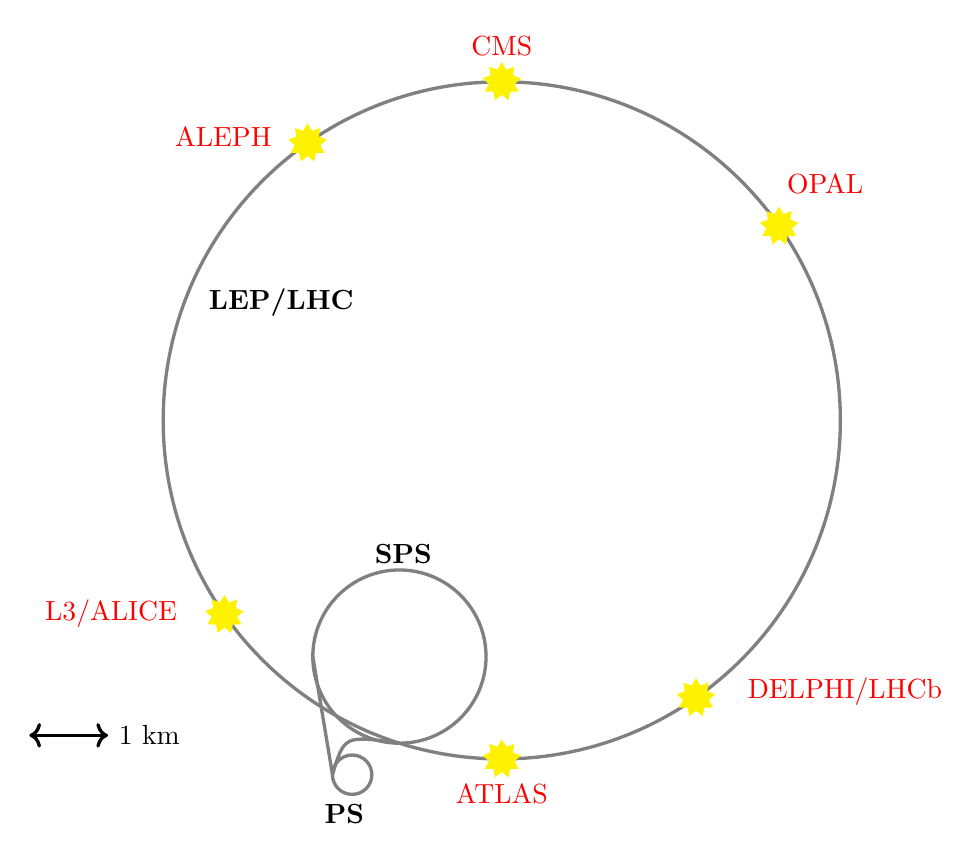
\begin{tikzpicture}[scale=1]
	\begin{scope}[shift={(0,0)}]

	    \draw[very thick, <->] (-6,-4) -- +(1,0) node[right] {1~km};

% LEP/LHC
	    \draw[very thick, color=gray] circle (4.3);
% SPS
	    \draw[very thick, color=gray] (-1.3,-3) circle (1.1);
% PS
	    \draw[very thick, color=gray] (-1.9,-4.5) circle (0.25);

	    \draw[very thick, color=gray] (-2.15,-4.5) -- (-2.4,-3);
	    \draw[very thick, color=gray] (-2.15,-4.5) .. controls (-2,-4) .. (-1.3,-4.1);

	   \foreach \x in {90,-90,35,125,215,305}
		    \node[fill,color=yellow,star,star points=9,minimum width=0.2] at ({4.3*cos(\x)},{4.3*sin(\x)}) (0.1) {};

	    \draw[red] node at (0,4.75) {CMS};
	    \draw[red] node at (0,-4.75) {ATLAS};
	    \draw[red] node[left] at (-4.,-2.45) {L3/ALICE};
	    \draw[red] node[right] at (3.,-3.45) {DELPHI/LHCb};
	    \draw[red] node[right] at (3.5,3.) {OPAL};
	    \draw[red] node[left] at (-2.8,3.6) {ALEPH};
	    \draw[black] node at (-2.8,1.5) {\textbf{LEP/LHC}};
	    \draw[black] node at (-1.25,-1.7) {\textbf{SPS}};
	    \draw[black] node at (-2,-5) {\textbf{PS}};
	\end{scope}
	    \end{tikzpicture}
	\caption{The layout of the LEP collider and the current CERN accelerators complex to operate the LHC (PS, SPS, and LHC drawn).
	During LEP time, four experiments -- ALEPH, DELPHI, L3, and OPAL -- were located in four interaction points. Currently,
	the ATLAS, CMS, LHCb, and ALICE experiments are located at the interaction points around the LHC ring.}
\end{center}
\end{figure}
%
%%%%%%%%%%%%%%%   END FIGURE  %%%%%%%%%%%%%%%%%%%%%%%%%%%%%%

\end{document}
